\section{Introducción}
El signo de Hoffmann es un reflejo muscular que se produce al percutir suavemente el lecho ungueal del dedo medio o índice como se muestra en la figura \ref{fig:Hoffman_sign}, produciéndose un movimiento de flexión involuntario del pulgar cuando el examinador hace girar la uña del dedo medio hacia abajo. Fue propuesto por primera vez por Johann Hoffmann, un neurólogo alemán, a finales del siglo XIX. Y descrito por primera vez gracias a Hans Curschmann, uno de sus asistentes, en 1911\cite{ BENDHEIM}. Su presencia puede indicar una lesión en los tractos corticoespinales, vías neuronales que conectan la corteza cerebral con la médula espinal. 


\begin{figure}[h!]
	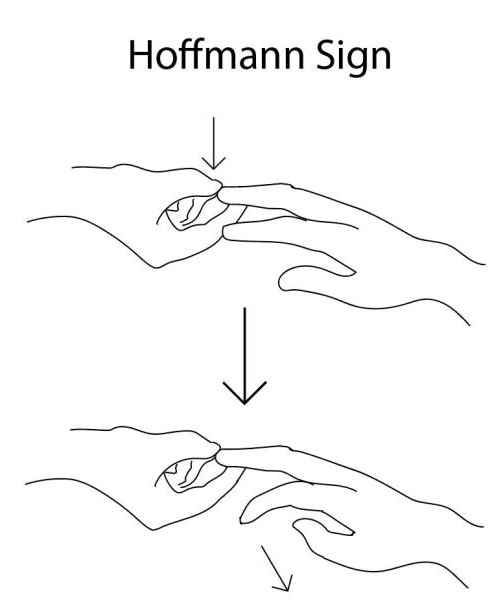
\includegraphics[width=0.35\textwidth]{figures/Kabir_Hoffmann__Sign.jpg}
	\caption{Signo de Hoffmann. Este diagrama muestra un signo de Hoffmann positivo, una parte estándar del examen neurológico común. Contribución de R Kabir, MD}
	\label{fig:Hoffman_sign}
\end{figure}


No obstante es importante destacar que el signo de Hoffman es un fenotipo y no una enfermedad en sí, se ha descubierto que hasta el 3\% de la población presenta un signo de Hoffmann positivo sin que haya compresión de la médula. Este reflejo está asociado a 12 enfermedades diferentes\cite{whitney}.

El signo de Hoffmann ha sido identificado en una serie de enfermedades neurodegenerativas y trastornos del tracto corticoespinal, muchas de ellas caracterizadas por alteraciones motoras progresivas. Entre estas patologías se encuentran diversas formas de paraplejía espástica hereditaria, son un grupo clínicamente y genéticamente heterogéneo de trastornos neurológicos, caracterizados principalmente por espasticidad progresiva y, a menudo, pérdida del sentido de la vibración en los miembros inferiores \cite{Esteves2014}, tanto autosómica dominante como recesiva. Por ejemplo, la paraplejía espástica 9A, de herencia autosómica dominante (OMIM:601162) \cite{10.1093/brain/awv143}, y las formas recesivas como la paraplejía espástica 72 (OMIM:615625), asociadas con disfunción motora grave.

Enfermedades neurodegenerativas más conocidas, como la esclerosis lateral amiotrófica (ORPHA:803), también muestran una asociación con el signo de Hoffmann, debido a la degeneración de las motoneuronas superiores \cite{RIANCHO201927}. Diversas formas de ataxias espásticas, relacionados con falta de coordinacion motora \cite{Pedroso2022}, como la ataxia espástica 9 (OMIM:618438) y 10 (OMIM:620666), completan el espectro de condiciones en las que este reflejo patológico se manifiesta.

A nivel molecular, diversos genes han sido asociados con condiciones que incluyen el signo de Hoffmann, reflejo que indica alteraciones en los tractos corticoespinales. Entre ellos, destacan SOD1, TARDBP y UBQLN2, los cuales están vinculados a la esclerosis lateral amiotrófica (ELA), una enfermedad neurodegenerativa que afecta las neuronas motoras superiores y provoca reflejos patológicos. Además, el gen NEK1 ha sido recientemente asociado con formas hereditarias de ELA, contribuyendo al deterioro de las vías motoras. Las mutaciones en estos genes interfieren con la función neuronal, causando degeneración progresiva en los tractos corticoespinales. Esto refuerza la relación entre el signo clínico de Hoffmann y la patología subyacente, ya que su presencia es un indicador importante del daño en las neuronas motoras superiores en estas enfermedades.